\section{Preliminary Study}

\andrew{
Most of these findings have come from preliminary interviews.
These should be replaced with findings from official formative interviews and studies.
}

We interviewed X programmers of varying backgrounds (novice, end user, professional).
We asked them questions including:
\begin{enumerate}
\item What resources do you use when figuring out how to code new tasks like the ones you just described?
\item Describe a time when you used a code example from the Internet in your program.  What was the coding task?  How and where did you find the code?
\end{enumerate}
We also asked users to specify how often (hourly, daily, weekly) that they used each of the web programming resources described by Parnin and Treude~\cite{Parnin-Measuring}, which include StackOverflow, blog-based tutorials, official API sites, forums, and mailing lists.
We also ask users about the frequency with which they accessed other resources, including books and internal source code.
We describe the following trends:

\subsection{What Resources Do Programmers Use in Active Periods?}
For the programmers we talked to, most used StackOverflow and official API sites on a daily basis.
About half of these users referenced forums and internal source code on a daily basis (see Figure~\ref{}).
All users explained that they frequently used Google to start searching for programming help.
We expect that many of them were directed to forums in most cases through a Google search.
Our interviewees used the remainder of web document types (other Q\&A sites besides StackOverflow, blog-based tutorials, books, mailing lists) only on a weekly basis or less often.
\andrew{TODO: break this down on a user-type basis.}

\begin{figure}
 \centering
 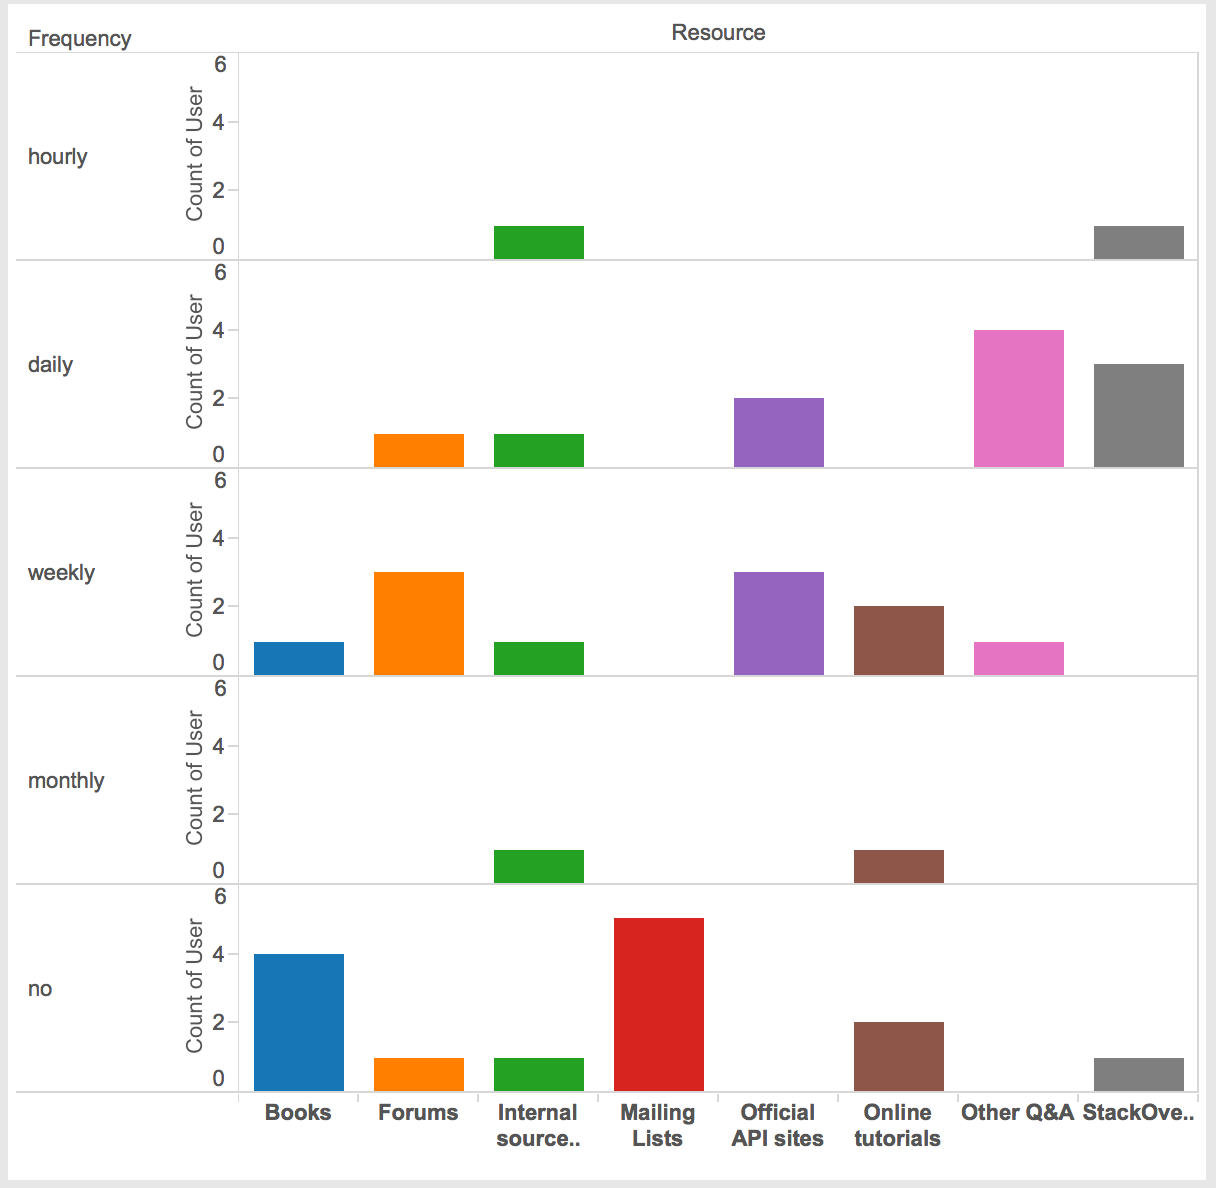
\includegraphics[width=.9\columnwidth]{figures/resource_frequencies}
 \caption{How often programmers use certain online resources when programming.}
 \label{fig:resource_frequencies}
\end{figure}

Of these resources, we consider \emph{wild code} to come from StackOverflow, forums, and tutorials.
We define wild code to be that which was not hand-developed by a software package's main developers.
\andrew{Caveat: some package developers do provide answers about their software StackOverflow.}
Wild code could also come from out-of-date or poorly-maintained API documentation.
Most large open source projects, we believe, do not post wild example code.

\subsection{Pitfalls of Using Wild Code}

The programmers we interviewed faced several challenges when working with wild code.

\emph{Unexpected runtime consequences}.
One professional programmer described copying a piece of code from online that used a thread pool.
The programmer altered the number of maximum threads that the pool could generate based on his intuition.
However, the team later discovered that this parameter resulted in a much longer runtime of the code when deployed.
It took the team several weeks to discover this error.
The programmer told us that if he had checked the \emph{Javadocs} documentation for this class, the appropriate parameters probably would have been selected before finishing integrating the snippet into code.

\emph{Unclear instructions}.
One programmer told us that the instructions for using a snippet online were not specific enough.
As a result, that individual spent extra time modifying the code to make it work.
Other times, usable API documentation may be missing altogether, which was the case for two of the issues programmers described.

\emph{Version problems}.
Two programmers mentioned that sometimes code that they discovered online was written to run for different versions of the package than the one they had.
One programmer mentioned that, when solving a programming problem, he found 3-5 examples related to the class functionality.
However, no single one of these examples represented the case he wanted to implement.
Furthermore, many of them used different versions of the same API.
So, he kept all examples open, using them to discover the correct sequence by picking and choosing from each of these examples.

\emph{Red herrings in finding bugs}.
One professional programmer we interviewed described a time when he copied code from an Internet source into his own code.
After refactoring the variable names in the snippet to match the correct symbols from his code, the program crashed.
After debugging, he discovered that there was a logical error.
However, this error was \emph{not} in the example code, but his original source code into which he copied the snippet.
Because the snippet came from an outside source, it was hard to determine whether the bug originated in this new code or the author's own code.

\emph{Wild code doesn't always follow best practices}.
Two programmers told us that although they found their eventual solution very quickly at first, they continued to flip through multiple pages of search results looking for alternatives.
The first result for both of them, which they ended up working with, did not follow best practices.
For one of the two programmers, it was only when he saw that this code was used in another location that he felt comfortable using it in his own code.
Both programmers eventually decided that they would rather complete the task with code that did not follow best practices than abandon solving the problem.

We aim to help users overcome the challenges of locating reliable, side effect-free code among the millions of programming examples available on the web.
